\documentclass[10pt,a4paper]{article}
\usepackage[utf8]{inputenc}
\usepackage[german]{babel}
\usepackage{amsmath}
\usepackage{amsfonts}
\usepackage{amssymb}
\usepackage{multirow}
\usepackage[left=2cm,right=2cm,top=2cm,bottom=2cm]{geometry}
\usepackage{wrapfig}
\usepackage{graphicx}
\usepackage{caption}
\usepackage[colorlinks]{hyperref}


\author{Christian Bespin \and Christopher Deutsch}
\title{Übungsblatt 1: Numerische Methoden der Physik}
\begin{document}
\maketitle

\section{Madelung-Konstante des NaCl-Kristalls}
\subsection{Physikalischer Hintergrund}
In einem Kristallgitter sind die Ionen durch elektrostatische Wechselwirkung
untereinander an den Kristall gebunden. Uns interessiert die durchschnittliche
potentielle Energie eines dieser Ionen (wird mit dem Index $i$ bezeichnet).
Diese entsteht in erster Näherung aus der Überlagerung der Coulomb-Potentiale
der Punktladungen im Kristallgefüge
(werden mit dem Index $j$ bezeichnet). Die Ladungszahl des jeweiligen Ions sei $z$
und $r_{ij}$ ist der Abstand des betrachteten Ionenpaars. Wir summieren für
jedes Ion des Kristalls (mit Ausnahme des $i$-Ions, da dessen Potential auf sich
selbst keinen Einfluss hat) den Beitrag zum Potential:

\begin{align}
\label{EPot}
E_G = \sum_{j\atop i \neq j} \frac{1}{4 \pi \epsilon_0}
\frac{z_i e \cdot z_j e}{r_{ij}}
\end{align}
Erweitern der Gleichung (\ref{EPot}) mit dem Gitterabstand $a$ und
Zusammenfassen des Faktors in die durchschnittliche Energie eines Ionenpaars
$E_P$ mit Abstand $a$ ergibt:

\begin{align}
E_G = \frac{1}{4 \pi \epsilon_0} \frac{e^2}{a} \sum_{j\atop i \neq j}
\frac{z_i z_j}{r_{ij}/a} = E_P \sum_{j\atop i \neq j} \frac{z_i z_j}{r_{ij}/a}
\end{align}
Schließlich wird die Geometrie des Kristalls in der Madelung-Konstante
zusammengefasst:

\begin{align}
\label{Madelungkonstante}
\alpha = \frac{E_G}{E_P} = \sum_{j\atop i \neq j} \frac{z_i z_j}{r_{ij}/a}
\end{align}
Dabei ist $r_{ij}/a$ der mit der Gitterkonstanten normalisierte Abstand der Ionen,
welcher im Folgenden ausschließlich für Längen verwendet wird.

\subsection{Algorithmus im 3-dimensionalen Fall}
\subsubsection{Struktur von Natriumchlorid}

Die nächsten Nachbarn eines jeden Ions sind sechs Ionen entgegengesetzter
Ladung. Diese Ionen befinden sich an den Eckpunkten eines regelmäßigen
Oktaeders. Dadurch kann das Vorzeichen der Ladung an der Gitterstelle
$\mathbf{r} = \left( x,y,z \right)$ relativ zu einer anderen Ladung durch:
\begin{align}
\mathrm{sgn}\left(z(\mathbf{r})\right) = \pm \left( -1 \right)^{x+y+z}
\label{eq:vorzeichen}
\end{align}
berechnet werden. Dabei wird das Vorzeichen so gewählt, dass dieses mit der Ladung
des Referenz-Ions übereinstimmt (Na: $+$; Cl: $-$). Diese Tatsache
äußert sich auch darin, dass das Vorzeichen der Madelung-Konstante vom
betrachteten Ion abhängt (generell: $\alpha_{Na} = - \alpha_{Cl}$).


\subsubsection{Probleme der naiven Methode}

Zunächst wurde die naive Implementierung analog zur mathematischen Beschreibung
getestet. Dabei wurde die Madelung-Konstante für einen Würfel analog zu
Gleichung (\ref{Madelungkonstante}), über sukzessive Erweiterung des Würfels um eine
Schale berechnet.Es fällt schnell die schlechte Konvergenz auf, die sich
physikalisch darin manifestiert, dass der Kristall, beim einfachen Erweitern
mit einer Schale, nicht elektrisch neutral bleibt.

\begin{wrapfigure}{R}[0pt]{0.47\textwidth}
	\vspace{-10pt}
	\centering
	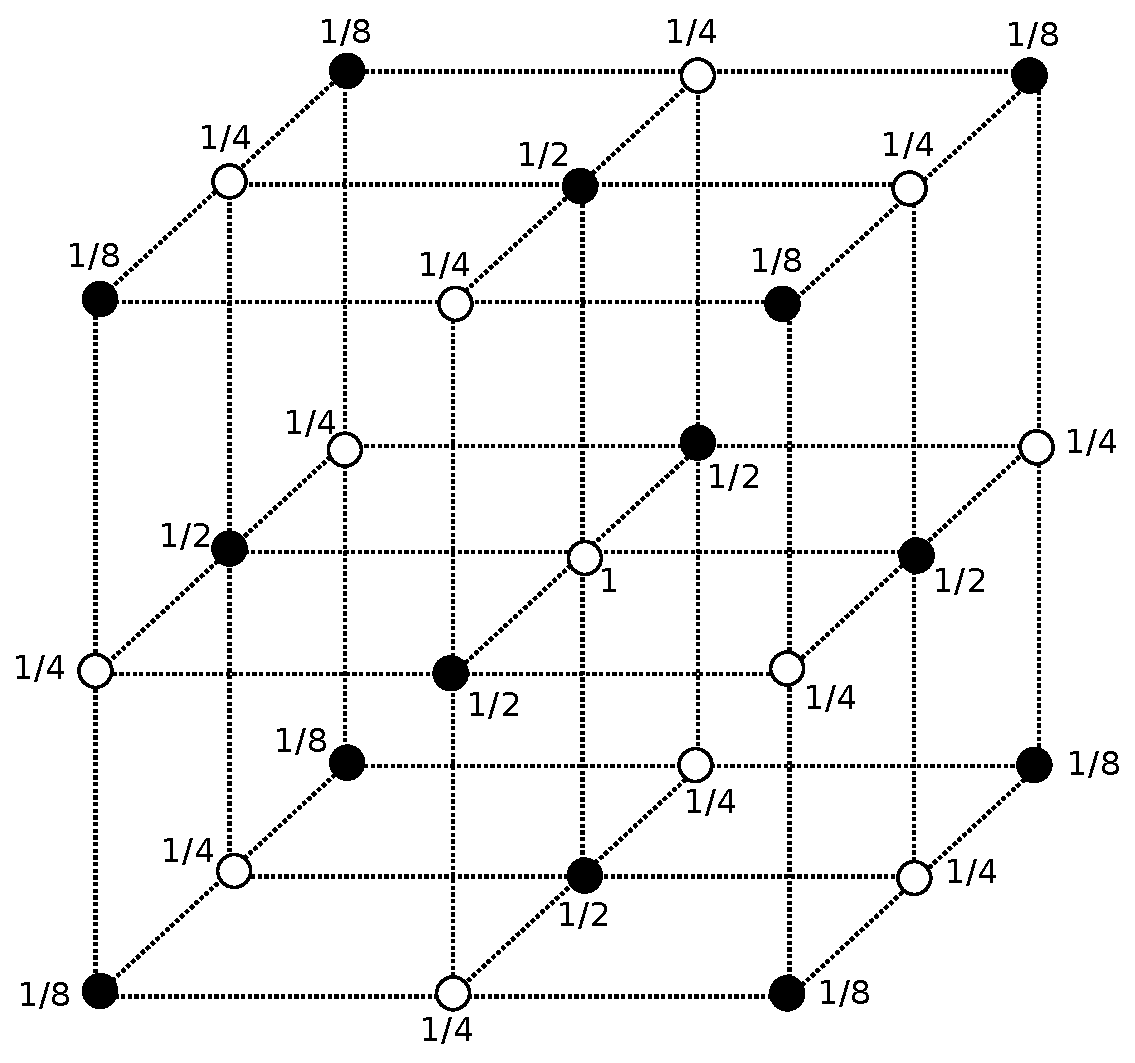
\includegraphics[width=0.35\textwidth]{./figures/wuerfel.eps}
	\caption{neutrale Elementarzelle nach Evjen}
	\label{skalierungsgrafik3d}
	\vspace{-20pt}
\end{wrapfigure}

Dieses Problem wurde von Evjen
\cite{Evjen} gelöst, indem er den Kristall in elektrisch neutrale Elementarzellen
aufteilt, die einen flacheren Potentialverlauf haben als einzelne Punktladungen.
Eine solche Zelle ist in Abbildung \ref{skalierungsgrafik3d} dargestellt,
dabei sind die gebrochenen Ladungen durch das Überlappen von mehreren Elementarzellen
motiviert (vgl. Abbildung \ref{zellensumme} für das zweidimensionale Analogon). Die Summe über 
alle Elementarzellen eines Würfels resultiert darin, dass die Ecken des Würfels
$\frac{1}{8}$, Kanten $\frac{1}{4}$ und Seitenflächen $\frac{1}{2}$ gewichtet werden
und der Innenraum voll in die Gewichtung eingeht.

\subsubsection{Beschreibung}

Der verwendete Algorithmus beginnt mit einem Ion im Koordinatenursprung. Dieses
erweitern wir schrittweise um eine Schale von Ionen mit den Ladungenzahlen gemäß
Gleichung (\ref{eq:vorzeichen}). Wir nutzen nun die Symmetrie des Würfels, um den Beitrag
der so konstruierten Schale zur Madelung-Konstante zu berechnen. Dazu teilen wir die
Schale in 8 symmetrisch äquivalente Ecken, 12 Kanten und 6 Seitenflächen auf, berechnen für
jeweils eines dieser Objekte den Beitrag zur Madelung-Konstante (nach Evjen gewichtet)
und multiplizieren mit dem entsprechenden Faktor. Dabei ist zu beachten, dass wir
den Rest der Gewichtung zwischenspeichern müssen, da nach dem Hinzufügen der nächsten
Schale die Ionen im Inneren des Würfels voll gewichtet werden (bei der nächsten Schale
wird dann einfach der Rest auf die Madelung-Konstante addiert). Diese Vorgehensweise ist notwendig, da wir das Verfahren solange wiederholen, bis die Differenz der Madelungkonstante
von zwei aufeinanderfolgenden Schalen kleiner als eine Zahl $0 < \epsilon < 1$ wird. Die
mathematische Relevanz dieser Abbruchbedingung wird in Abschnitt \ref{sssec:Konvergenz}
erklärt.

\subsubsection{Konvergenz}

\label{sssec:Konvergenz}
\vspace{-10pt}
\begin{figure}[h]
\begin{minipage}[c]{0.5\textwidth}
\captionsetup{type=figure}
\begin{center}
% GNUPLOT: LaTeX picture with Postscript
\begingroup
  \makeatletter
  \providecommand\color[2][]{%
    \GenericError{(gnuplot) \space\space\space\@spaces}{%
      Package color not loaded in conjunction with
      terminal option `colourtext'%
    }{See the gnuplot documentation for explanation.%
    }{Either use 'blacktext' in gnuplot or load the package
      color.sty in LaTeX.}%
    \renewcommand\color[2][]{}%
  }%
  \providecommand\includegraphics[2][]{%
    \GenericError{(gnuplot) \space\space\space\@spaces}{%
      Package graphicx or graphics not loaded%
    }{See the gnuplot documentation for explanation.%
    }{The gnuplot epslatex terminal needs graphicx.sty or graphics.sty.}%
    \renewcommand\includegraphics[2][]{}%
  }%
  \providecommand\rotatebox[2]{#2}%
  \@ifundefined{ifGPcolor}{%
    \newif\ifGPcolor
    \GPcolortrue
  }{}%
  \@ifundefined{ifGPblacktext}{%
    \newif\ifGPblacktext
    \GPblacktextfalse
  }{}%
  % define a \g@addto@macro without @ in the name:
  \let\gplgaddtomacro\g@addto@macro
  % define empty templates for all commands taking text:
  \gdef\gplbacktext{}%
  \gdef\gplfronttext{}%
  \makeatother
  \ifGPblacktext
    % no textcolor at all
    \def\colorrgb#1{}%
    \def\colorgray#1{}%
  \else
    % gray or color?
    \ifGPcolor
      \def\colorrgb#1{\color[rgb]{#1}}%
      \def\colorgray#1{\color[gray]{#1}}%
      \expandafter\def\csname LTw\endcsname{\color{white}}%
      \expandafter\def\csname LTb\endcsname{\color{black}}%
      \expandafter\def\csname LTa\endcsname{\color{black}}%
      \expandafter\def\csname LT0\endcsname{\color[rgb]{1,0,0}}%
      \expandafter\def\csname LT1\endcsname{\color[rgb]{0,1,0}}%
      \expandafter\def\csname LT2\endcsname{\color[rgb]{0,0,1}}%
      \expandafter\def\csname LT3\endcsname{\color[rgb]{1,0,1}}%
      \expandafter\def\csname LT4\endcsname{\color[rgb]{0,1,1}}%
      \expandafter\def\csname LT5\endcsname{\color[rgb]{1,1,0}}%
      \expandafter\def\csname LT6\endcsname{\color[rgb]{0,0,0}}%
      \expandafter\def\csname LT7\endcsname{\color[rgb]{1,0.3,0}}%
      \expandafter\def\csname LT8\endcsname{\color[rgb]{0.5,0.5,0.5}}%
    \else
      % gray
      \def\colorrgb#1{\color{black}}%
      \def\colorgray#1{\color[gray]{#1}}%
      \expandafter\def\csname LTw\endcsname{\color{white}}%
      \expandafter\def\csname LTb\endcsname{\color{black}}%
      \expandafter\def\csname LTa\endcsname{\color{black}}%
      \expandafter\def\csname LT0\endcsname{\color{black}}%
      \expandafter\def\csname LT1\endcsname{\color{black}}%
      \expandafter\def\csname LT2\endcsname{\color{black}}%
      \expandafter\def\csname LT3\endcsname{\color{black}}%
      \expandafter\def\csname LT4\endcsname{\color{black}}%
      \expandafter\def\csname LT5\endcsname{\color{black}}%
      \expandafter\def\csname LT6\endcsname{\color{black}}%
      \expandafter\def\csname LT7\endcsname{\color{black}}%
      \expandafter\def\csname LT8\endcsname{\color{black}}%
    \fi
  \fi
  \setlength{\unitlength}{0.0500bp}%
  \begin{picture}(5040.00,3024.00)%
    \gplgaddtomacro\gplbacktext{%
      \csname LTb\endcsname%
      \put(1474,704){\makebox(0,0)[r]{\strut{} 1.74745}}%
      \put(1474,1047){\makebox(0,0)[r]{\strut{} 1.7475}}%
      \put(1474,1389){\makebox(0,0)[r]{\strut{} 1.74755}}%
      \put(1474,1732){\makebox(0,0)[r]{\strut{} 1.7476}}%
      \put(1474,2074){\makebox(0,0)[r]{\strut{} 1.74765}}%
      \put(1474,2417){\makebox(0,0)[r]{\strut{} 1.7477}}%
      \put(1474,2759){\makebox(0,0)[r]{\strut{} 1.74775}}%
      \put(2040,484){\makebox(0,0){\strut{} 5}}%
      \put(3125,484){\makebox(0,0){\strut{} 10}}%
      \put(4209,484){\makebox(0,0){\strut{} 15}}%
      \put(176,1731){\rotatebox{-270}{\makebox(0,0){\strut{}Madelungkonstante $\tilde{\alpha}(n)$}}}%
      \put(3124,154){\makebox(0,0){\strut{}Anzahl hinzugef\"{u}gter Schalen n}}%
      \put(3124,2649){\makebox(0,0){\strut{}}}%
    }%
    \gplgaddtomacro\gplfronttext{%
      \csname LTb\endcsname%
      \put(3656,2586){\makebox(0,0)[r]{\strut{}\footnotesize Madelung-Konstante}}%
      \csname LTb\endcsname%
      \put(3656,2366){\makebox(0,0)[r]{\strut{}\footnotesize Literaturwert}}%
    }%
    \gplbacktext
    \put(0,0){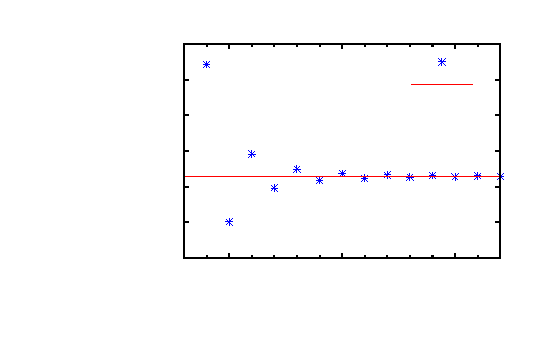
\includegraphics{ergebnis}}%
    \gplfronttext
  \end{picture}%
\endgroup

\caption{Grafische Darstellung der Konvergenz}
\label{plotkonvergenz3d}
\end{center}
\end{minipage}
\begin{minipage}[c]{0.5\textwidth}
\captionsetup{type=table}
\begin{center}
\begin{tabular}{c|c|c}
\rule[-1ex]{0pt}{2.5ex} $n$ & $\tilde{\alpha}(n)$ & $\delta_\alpha$ \\ 
\hline 
\rule[-1ex]{0pt}{2.5ex} $1$ & $1.456029925630$ & $1.67\cdot10^{-1}$ \\ 
\hline 
\rule[-1ex]{0pt}{2.5ex} $2$ & $1.751769133337$ & $2.41\cdot10^{-3}$ \\ 
\hline
\rule[-1ex]{0pt}{2.5ex} $5$ & $1.747500502341$ & $3.67\cdot10^{-5}$ \\ 
\hline 
\rule[-1ex]{0pt}{2.5ex} $10$ & $1.747568603772$ & $2.29\cdot10^{-6}$ \\ 
\hline 
\rule[-1ex]{0pt}{2.5ex} $20$ & $1.747564845218$ & $1.43\cdot10^{-7}$ \\ 
\hline 
\rule[-1ex]{0pt}{2.5ex} $50$ & $1.747564601048$ & $3.67\cdot10^{-9}$ \\
\hline
\rule[-1ex]{0pt}{2.5ex} $100$ & $1.747564595034$ & $2.30\cdot10^{-10}$ \\ 
\hline
\rule[-1ex]{0pt}{2.5ex} $200$ & $1.747564594660$ & $1.51\cdot10^{-11}$ \\ 
\hline
\rule[1ex]{0pt}{2.5ex} Lit. & $1.747564694633$ & $ - $
\end{tabular}
\captionof{table}{Anzahl der hinzugefügten Schalen $n$ gegen Madelung-Konstante $\tilde{\alpha}(n)$ nach $n$ Iterationen des Algorithmus und relativer Fehler $\delta_\alpha$}
\label{tab:konvergenz3d}
\end{center}
\end{minipage}
\end{figure}

Im Folgenden bezeichnet $\alpha$ den wahren Wert der Madelung-Konstante
und $\tilde{\alpha}(n)$ die nach unserem Algorithmus berechnete Madelung-Konstante
nach $n$ Iterationen.
In Tabelle \ref{tab:konvergenz3d} wurde die Anzahl der hinzugefügten Schalen $n$
gegen den Wert der Madelung-Konstante $\tilde{\alpha}(n)$ und den relativen Fehler $\delta_\alpha$ zum
Literaturwert $\alpha = 1.7475646946331822$ \cite{Sakamoto} aufgetragen.
Wie man sieht, ist die Abweichung vom Literaturwert schon nach wenigen Iterationen
sehr klein.
Man sieht ebenfalls (Abbildung \ref{plotkonvergenz3d}), dass der berechnete Wert
der Madelung-Konstante mit steigenden $n$ und fallendem absoluten Fehler $\Delta_\alpha$ um
den wahren Wert alterniert. Der absolute Fehler ist also:
\begin{align}
	\Delta_\alpha = | \tilde{\alpha}(n) - \alpha | \leq | \tilde{\alpha}(n) - \tilde{\alpha}(n-1)| < \epsilon
\end{align}
Dies rechtfertigt unser Abbruchkriterium, denn es ist garantiert, dass beim Eintreten der
Abbruchbedingung der absolute Fehler $\Delta_\alpha$ kleiner als $\epsilon$ ist.
Außerdem gilt $\alpha > 1$, sodass für den relativen Fehler $\delta_\alpha$ folgt:
\begin{align}
	\delta_\alpha = \frac{\Delta_\alpha}{\alpha} < \epsilon
\end{align}

\subsection{Algorithmus im 2-dimensionalen Fall}
\subsubsection{Beschreibung}
Um die Methode von Evjen auf den zweidimensionalen Fall zu übertragen, sieht man leicht,
dass um elektrische Neutralität einer Elementarzelle zu erreichen, die Ecken mit $\frac{1}{4}$
und die Kanten mit $\frac{1}{2}$ gewichtet werden müssen (Abbildung \ref{skalierungsgrafik2d}).
Die Summe über alle Elementarzellen führt analog zum 3-dimensionalen Fall dazu, dass die Ecken
des Quadrates $\frac{1}{4}$ und die Kanten $\frac{1}{2}$ (Abbildung \ref{zellensumme}).
Die Vorgehensweise ist analog zum 3-dimensionalen Fall, mit Ausnahme der Abbruchbedingung.
Der Wert der Madelungkonstante alterniert in diesem Fall nicht um den wahren Wert (vgl. Abbildung \ref{plotkonvergenz2d}), weshalb
wir einen direkten Vergleich mit dem Literaturwert durchführen. Die Funktion wird beendet
sobald absolute Fehler $\Delta_\alpha$ einen vorgegebenen Wert $\epsilon$ unterschreitet.

\vspace{\baselineskip}
\begin{minipage}[c]{0.5\textwidth}
\captionsetup{type=figure}
\begin{center}
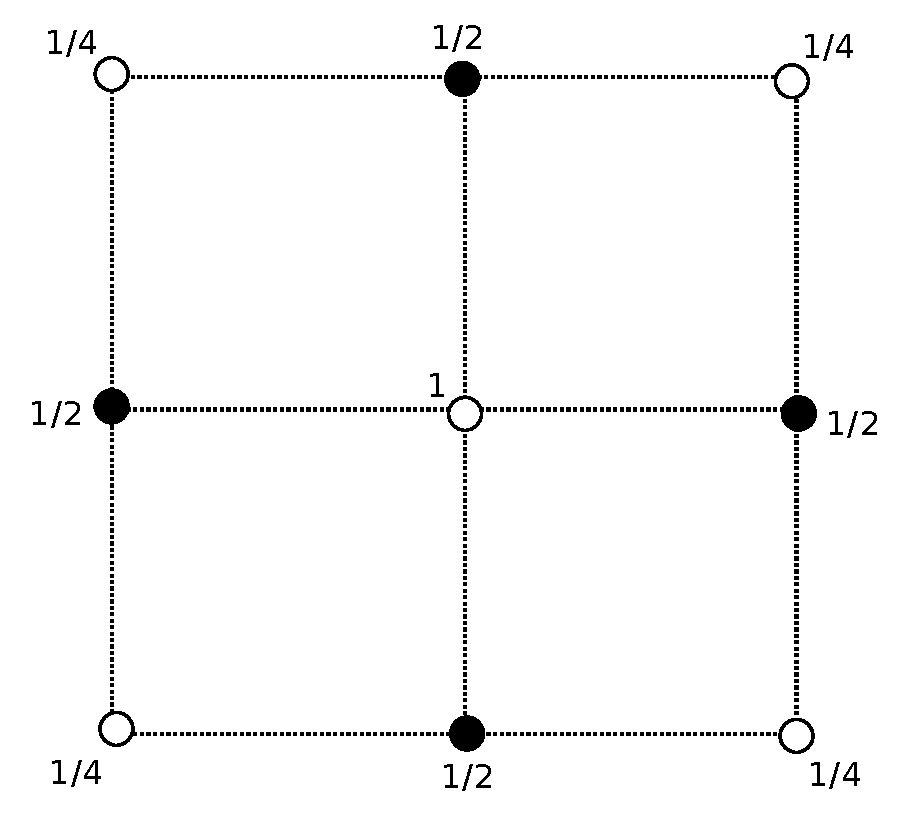
\includegraphics[height=0.5\textwidth]{./figures/quadrat.eps}
\caption{neutrale Elementarzelle (2-dim.)}
\label{skalierungsgrafik2d}
\end{center}
\end{minipage}
\begin{minipage}[c]{0.5\textwidth}
\captionsetup{type=figure}
\begin{center}
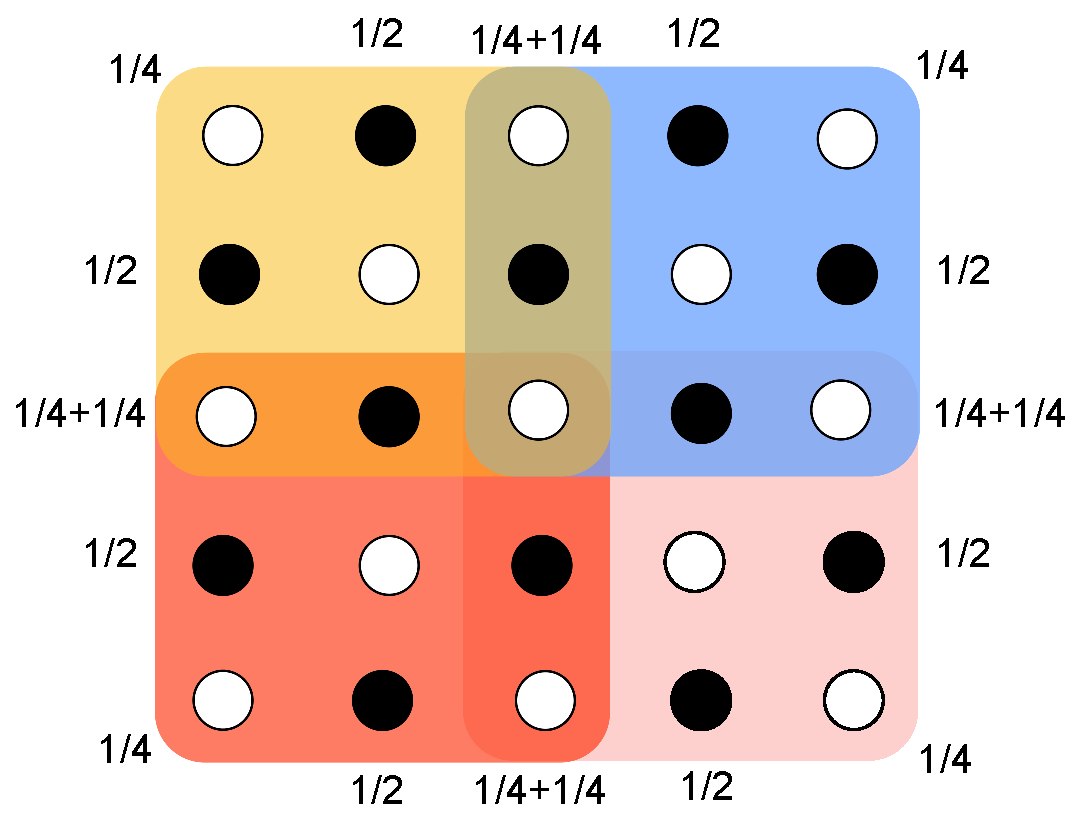
\includegraphics[height=0.5\textwidth]{./figures/elementarzelle.eps}
\caption{Aneinanderreihung von Elementarzellen}
\label{zellensumme}
\end{center}
\end{minipage}	

\subsubsection{Konvergenz}

\vspace{-10pt}
\begin{figure}[h]
\begin{minipage}[c]{0.5\textwidth}
\captionsetup{type=figure}
\begin{center}
% GNUPLOT: LaTeX picture with Postscript
\begingroup
  \makeatletter
  \providecommand\color[2][]{%
    \GenericError{(gnuplot) \space\space\space\@spaces}{%
      Package color not loaded in conjunction with
      terminal option `colourtext'%
    }{See the gnuplot documentation for explanation.%
    }{Either use 'blacktext' in gnuplot or load the package
      color.sty in LaTeX.}%
    \renewcommand\color[2][]{}%
  }%
  \providecommand\includegraphics[2][]{%
    \GenericError{(gnuplot) \space\space\space\@spaces}{%
      Package graphicx or graphics not loaded%
    }{See the gnuplot documentation for explanation.%
    }{The gnuplot epslatex terminal needs graphicx.sty or graphics.sty.}%
    \renewcommand\includegraphics[2][]{}%
  }%
  \providecommand\rotatebox[2]{#2}%
  \@ifundefined{ifGPcolor}{%
    \newif\ifGPcolor
    \GPcolortrue
  }{}%
  \@ifundefined{ifGPblacktext}{%
    \newif\ifGPblacktext
    \GPblacktextfalse
  }{}%
  % define a \g@addto@macro without @ in the name:
  \let\gplgaddtomacro\g@addto@macro
  % define empty templates for all commands taking text:
  \gdef\gplbacktext{}%
  \gdef\gplfronttext{}%
  \makeatother
  \ifGPblacktext
    % no textcolor at all
    \def\colorrgb#1{}%
    \def\colorgray#1{}%
  \else
    % gray or color?
    \ifGPcolor
      \def\colorrgb#1{\color[rgb]{#1}}%
      \def\colorgray#1{\color[gray]{#1}}%
      \expandafter\def\csname LTw\endcsname{\color{white}}%
      \expandafter\def\csname LTb\endcsname{\color{black}}%
      \expandafter\def\csname LTa\endcsname{\color{black}}%
      \expandafter\def\csname LT0\endcsname{\color[rgb]{1,0,0}}%
      \expandafter\def\csname LT1\endcsname{\color[rgb]{0,1,0}}%
      \expandafter\def\csname LT2\endcsname{\color[rgb]{0,0,1}}%
      \expandafter\def\csname LT3\endcsname{\color[rgb]{1,0,1}}%
      \expandafter\def\csname LT4\endcsname{\color[rgb]{0,1,1}}%
      \expandafter\def\csname LT5\endcsname{\color[rgb]{1,1,0}}%
      \expandafter\def\csname LT6\endcsname{\color[rgb]{0,0,0}}%
      \expandafter\def\csname LT7\endcsname{\color[rgb]{1,0.3,0}}%
      \expandafter\def\csname LT8\endcsname{\color[rgb]{0.5,0.5,0.5}}%
    \else
      % gray
      \def\colorrgb#1{\color{black}}%
      \def\colorgray#1{\color[gray]{#1}}%
      \expandafter\def\csname LTw\endcsname{\color{white}}%
      \expandafter\def\csname LTb\endcsname{\color{black}}%
      \expandafter\def\csname LTa\endcsname{\color{black}}%
      \expandafter\def\csname LT0\endcsname{\color{black}}%
      \expandafter\def\csname LT1\endcsname{\color{black}}%
      \expandafter\def\csname LT2\endcsname{\color{black}}%
      \expandafter\def\csname LT3\endcsname{\color{black}}%
      \expandafter\def\csname LT4\endcsname{\color{black}}%
      \expandafter\def\csname LT5\endcsname{\color{black}}%
      \expandafter\def\csname LT6\endcsname{\color{black}}%
      \expandafter\def\csname LT7\endcsname{\color{black}}%
      \expandafter\def\csname LT8\endcsname{\color{black}}%
    \fi
  \fi
  \setlength{\unitlength}{0.0500bp}%
  \begin{picture}(5040.00,3024.00)%
    \gplgaddtomacro\gplbacktext{%
      \csname LTb\endcsname%
      \put(1078,704){\makebox(0,0)[r]{\strut{} 1.25}}%
      \put(1078,961){\makebox(0,0)[r]{\strut{} 1.3}}%
      \put(1078,1218){\makebox(0,0)[r]{\strut{} 1.35}}%
      \put(1078,1475){\makebox(0,0)[r]{\strut{} 1.4}}%
      \put(1078,1732){\makebox(0,0)[r]{\strut{} 1.45}}%
      \put(1078,1988){\makebox(0,0)[r]{\strut{} 1.5}}%
      \put(1078,2245){\makebox(0,0)[r]{\strut{} 1.55}}%
      \put(1078,2502){\makebox(0,0)[r]{\strut{} 1.6}}%
      \put(1078,2759){\makebox(0,0)[r]{\strut{} 1.65}}%
      \put(1210,484){\makebox(0,0){\strut{} 0}}%
      \put(2354,484){\makebox(0,0){\strut{} 5}}%
      \put(3499,484){\makebox(0,0){\strut{} 10}}%
      \put(4643,484){\makebox(0,0){\strut{} 15}}%
      \put(176,1731){\rotatebox{-270}{\makebox(0,0){\strut{}Madelung-Konstante $\tilde{\alpha}$}}}%
      \put(2926,154){\makebox(0,0){\strut{}Anzahl hinzugef\"{u}gter Schalen n}}%
      \put(2926,2649){\makebox(0,0){\strut{}}}%
    }%
    \gplgaddtomacro\gplfronttext{%
      \csname LTb\endcsname%
      \put(3656,1097){\makebox(0,0)[r]{\strut{}\footnotesize Madelung-Konstante $\tilde{\alpha}$}}%
      \csname LTb\endcsname%
      \put(3656,877){\makebox(0,0)[r]{\strut{}\footnotesize Literaturwert ${\alpha}$}}%
    }%
    \gplbacktext
    \put(0,0){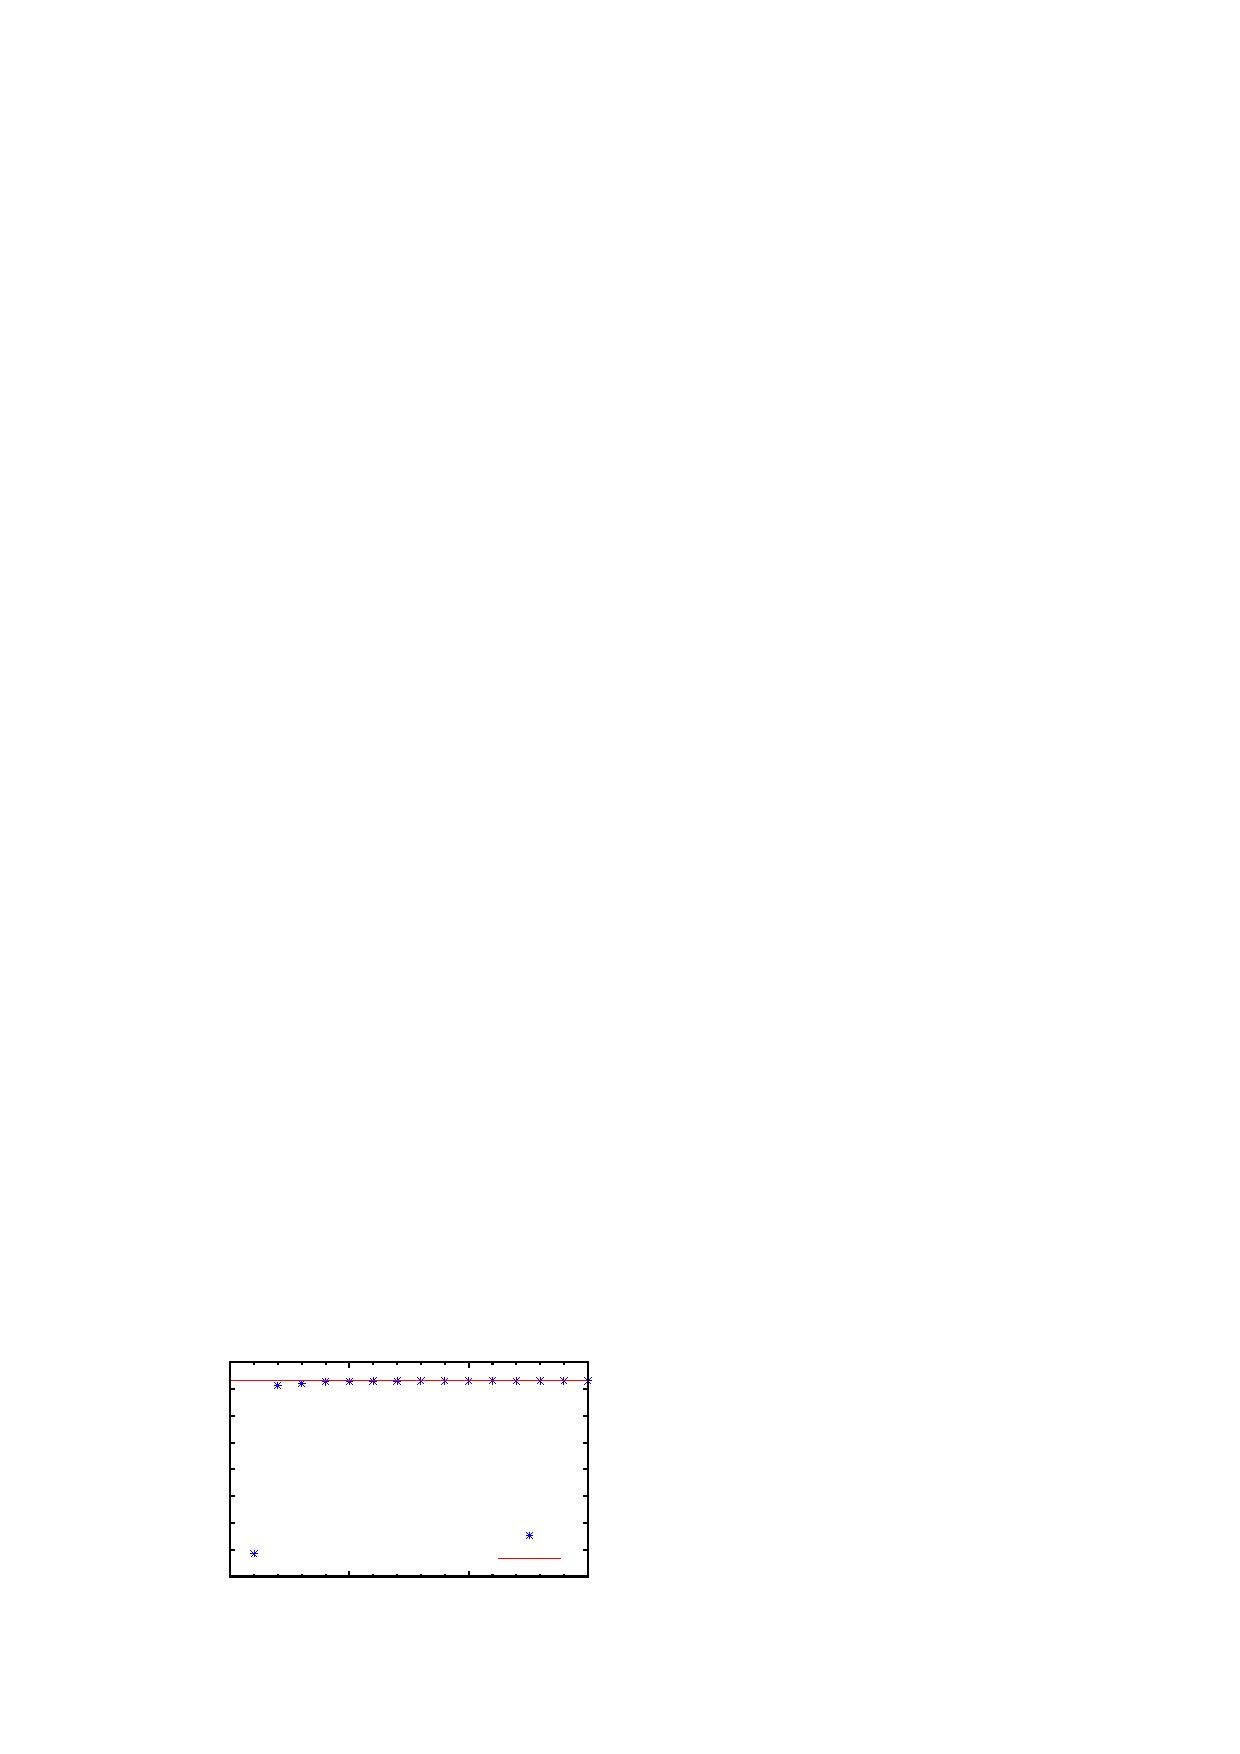
\includegraphics{./figures/ergebnis2d}}%
    \gplfronttext
  \end{picture}%
\endgroup

\caption{Grafische Darstellung der 2-dim. Konvergenz}
\label{plotkonvergenz2d}
\end{center}
\end{minipage}
\begin{minipage}[c]{0.5\textwidth}
\captionsetup{type=table}
\begin{center}
\begin{tabular}{c|c|c}
\rule[-1ex]{0pt}{2.5ex} $n$ & $\tilde{\alpha}(n)$ & $\delta_\alpha$ \\ 
\hline 
\rule[-1ex]{0pt}{2.5ex} $1$ & $1.292893218813$ & $2.00\cdot10^{-1}$ \\ 
\hline 
\rule[-1ex]{0pt}{2.5ex} $2$ & $1.606873866660$ & $5.37\cdot10^{-3}$ \\ 
\hline
\rule[-1ex]{0pt}{2.5ex} $5$ & $1.614491025405$ & $6.51\cdot10^{-4}$ \\ 
\hline 
\rule[-1ex]{0pt}{2.5ex} $10$ & $1.615410325066$ & $8.19\cdot10^{-5}$ \\ 
\hline 
\rule[-1ex]{0pt}{2.5ex} $20$ & $1.615526062566$ & $1.03\cdot10^{-5}$ \\ 
\hline 
\rule[-1ex]{0pt}{2.5ex} $50$ & $1.615541566141$ & $6.56\cdot10^{-7}$ \\
\hline
\rule[-1ex]{0pt}{2.5ex} $100$ & $1.615542494133$ & $8.21\cdot10^{-8}$ \\ 
\hline
\rule[-1ex]{0pt}{2.5ex} $200$ & $1.615542610140$ & $1.03\cdot10^{-8}$ \\ 
\hline
\rule[1ex]{0pt}{2.5ex} Lit.   & $1.615542626713$ & $ - $
\end{tabular}
\captionof{table}{Anzahl der hinzugefügten Schalen $n$ gegen Madelung-Konstante $\tilde{\alpha}(n)$ nach $n$ Iterationen des Algorithmus und relativer Fehler $\delta_\alpha$}
\label{tab:konvergenz2d}
\end{center}
\end{minipage}
\end{figure}
Wegen $\alpha > 1$ garantiert die gewählte Abbruchbedingung (der absolute Fehler $\Delta_\alpha$ ist kleiner als $\epsilon > 0$), 
dass der relative Fehler $\delta_\alpha < \epsilon$ ist. Der hier angenommene Literaturwert ist $\alpha = 1.6155426267128247$\footnote{\href{https://oeis.org/A088537}{A088537} \emph{Decimal expansion of Madelung's constant M2}, \textbf{The On-Line Encyclopedia of Integer Sequences}}. Tabelle \ref{tab:konvergenz2d} ist zu entnehmen, dass der Algorithmus, ähnlich wie im dreidimensionalen Fall, auch schnell konvergiert, wenn auch etwas langsamer. Dies relativiert sich dadurch, dass im Zweidimensionalen
nicht soviele Operationen durchgeführt werden müssen, wie im Dreidimensionalen.

\subsection{Fazit}

\begin{wraptable}{R}[0pt]{0.47\textwidth}
\begin{tabular}{|c|c|c|c|}
\hline
Fall & $\epsilon$                       & $\tilde{\alpha}$ & $\delta_\alpha$    \\ \hline
2D   & \multirow{2}{*}{$1\cdot10^{-5}$} & $1.615533039442$ & $5.93\cdot10^{-6}$ \\ \cline{1-1} \cline{3-4} 
3D   &                                  & $1.747561856286$ & $1.57\cdot10^{-6}$ \\ \hline
\end{tabular}
\caption{Ausgabe unseres Programmes bei vorgegebener Genauigkeit $\epsilon$}
\label{tab:ausgabe}
\end{wraptable}

Lorem ipsum dolor sit amet,\ref{tab:ausgabe} consetetur sadipscing elitr, sed diam nonumy eirmod tempor invidunt ut labore et dolore magna aliquyam erat, sed diam voluptua. At vero eos et accusam et justo duo dolores et ea rebum. Stet clita kasd gubergren, no sea takimata sanctus est Lorem ipsum dolor sit amet. Lorem ipsum dolor sit amet, consetetur sadipscing elitr, sed diam nonumy eirmod tempor invidunt ut labore et dolore magna aliquyam erat, sed diam voluptua. At vero eos et accusam et justo duo dolores et ea rebum. Stet clita kasd gubergren, no sea takimata sanctus est Lorem ipsum dolor sit amet.

\begin{thebibliography}{9}

\bibitem{Evjen}
Evjen, H. M.
\emph{On the Stability of Certain Heteropolar Crystals},
Physical Review Letters \textbf{39},
675-687 (1932)

\bibitem{Sakamoto}
Sakamoto, Y.
\emph{Madelung Constants of Simple Crystals Expressed in Terms of Born's Basic
Potentials of 15 Figures},
The Journal of Chemical Physics \textbf{28},
164 (1958)

\end{thebibliography}

\end{document}
